\documentclass[11pt,letterpaper]{article}
\usepackage[utf8]{inputenc}
\usepackage[left=1in,right=1in,top=1in,bottom=1in]{geometry}
\usepackage{amsfonts,amsmath}
\usepackage{graphicx,float}
% -----------------------------------
\usepackage{hyperref}
\hypersetup{%
  colorlinks=true,
  linkcolor=blue,
  citecolor=blue,
  urlcolor=blue,
  linkbordercolor={0 0 1}
}
% -----------------------------------
\usepackage{fancyhdr}
\newcommand\course{Numerical Analysis}
\newcommand\hwnumber{2}                  % <-- homework number
\newcommand\NetIDa{Ryan Sh\`iji\'e D\`u} 
\newcommand\NetIDb{September 23rd, 2022}
\pagestyle{fancyplain}
\headheight 35pt
\lhead{\NetIDa\\\NetIDb}
\chead{\textbf{\Large Worksheet \hwnumber}}
\rhead{\course}
\lfoot{}
\cfoot{}
\rfoot{\small\thepage}
\headsep 1.5em
% -----------------------------------
\usepackage{titlesec}
\renewcommand\thesubsection{(\arabic{section}.\alph{subsection})}
\titleformat{\subsection}[runin]
        {\normalfont\bfseries}
        {\thesubsection}% the label and number
        {0.5em}% space between label/number and subsection title
        {}% formatting commands applied just to subsection title
        []% punctuation or other commands following subsection title
% -----------------------------------
\setlength{\parindent}{0.0in}
\setlength{\parskip}{0.1in}
% -----------------------------------
\newcommand{\de}{\mathrm{d}}
\newcommand{\DD}{\mathrm{D}}
\newcommand{\pe}{\partial}
\newcommand{\mcal}{\mathcal}
%\newcommand{\pdx}{\left|\frac{\partial}{\partial_x}\right|}

\newcommand{\dsp}{\displaystyle}

\newcommand{\norm}[1]{\left\Vert #1 \right\Vert}
%\newcommand{\mean}[1]{\left\langle #1 \right\rangle}
\newcommand{\mean}[1]{\overline{#1}}
\newcommand{\inner}[2]{\left\langle #1,#2\right\rangle}

\newcommand{\ve}[1]{\boldsymbol{#1}}

\newcommand{\thus}{\Rightarrow \quad }
\newcommand{\fff}{\iff\quad}
\newcommand{\qdt}[1]{\quad \mbox{#1} \quad}

\renewcommand{\Re}{\mathrm{Re}}
\renewcommand{\Im}{\mathrm{Im}}
\newcommand{\E}{\mathbb{E}}
\newcommand{\lap} {\nabla^2}
\renewcommand{\div}{\nabla\cdot}

\newcommand{\csch}{\text{csch}}
\newcommand{\sech}{\text{sech}}


\newcommand{\hot}{\text{h.o.t.}}

\newcommand{\ssp}{\left.\qquad\right.}

\newcommand{\var}{\text{var}}
\newcommand{\cov}{\text{cov}}

%%%%%%%%%%%%%%%%%%%%%%%%%%%%%%%%%%%%%%%%%%%%%%%%%%
\makeatletter
\newcommand*{\mint}[1]{%
  % #1: overlay symbol
  \mint@l{#1}{}%
}
\newcommand*{\mint@l}[2]{%
  % #1: overlay symbol
  % #2: limits
  \@ifnextchar\limits{%
    \mint@l{#1}%
  }{%
    \@ifnextchar\nolimits{%
      \mint@l{#1}%
    }{%
      \@ifnextchar\displaylimits{%
        \mint@l{#1}%
      }{%
        \mint@s{#2}{#1}%
      }%
    }%
  }%
}
\newcommand*{\mint@s}[2]{%
  % #1: limits
  % #2: overlay symbol
  \@ifnextchar_{%
    \mint@sub{#1}{#2}%
  }{%
    \@ifnextchar^{%
      \mint@sup{#1}{#2}%
    }{%
      \mint@{#1}{#2}{}{}%
    }%
  }%
}
\def\mint@sub#1#2_#3{%
  \@ifnextchar^{%
    \mint@sub@sup{#1}{#2}{#3}%
  }{%
    \mint@{#1}{#2}{#3}{}%
  }%
}
\def\mint@sup#1#2^#3{%
  \@ifnextchar_{%
    \mint@sup@sub{#1}{#2}{#3}%
  }{%
    \mint@{#1}{#2}{}{#3}%
  }%
}
\def\mint@sub@sup#1#2#3^#4{%
  \mint@{#1}{#2}{#3}{#4}%
}
\def\mint@sup@sub#1#2#3_#4{%
  \mint@{#1}{#2}{#4}{#3}%
}
\newcommand*{\mint@}[4]{%
  % #1: \limits, \nolimits, \displaylimits
  % #2: overlay symbol: -, =, ...
  % #3: subscript
  % #4: superscript
  \mathop{}%
  \mkern-\thinmuskip
  \mathchoice{%
    \mint@@{#1}{#2}{#3}{#4}%
        \displaystyle\textstyle\scriptstyle
  }{%
    \mint@@{#1}{#2}{#3}{#4}%
        \textstyle\scriptstyle\scriptstyle
  }{%
    \mint@@{#1}{#2}{#3}{#4}%
        \scriptstyle\scriptscriptstyle\scriptscriptstyle
  }{%
    \mint@@{#1}{#2}{#3}{#4}%
        \scriptscriptstyle\scriptscriptstyle\scriptscriptstyle
  }%
  \mkern-\thinmuskip
  \int#1%
  \ifx\\#3\\\else_{#3}\fi
  \ifx\\#4\\\else^{#4}\fi  
}
\newcommand*{\mint@@}[7]{%
  % #1: limits
  % #2: overlay symbol
  % #3: subscript
  % #4: superscript
  % #5: math style
  % #6: math style for overlay symbol
  % #7: math style for subscript/superscript
  \begingroup
    \sbox0{$#5\int\m@th$}%
    \sbox2{$#5\int_{}\m@th$}%
    \dimen2=\wd0 %
    % => \dimen2 = width of \int
    \let\mint@limits=#1\relax
    \ifx\mint@limits\relax
      \sbox4{$#5\int_{\kern1sp}^{\kern1sp}\m@th$}%
      \ifdim\wd4>\wd2 %
        \let\mint@limits=\nolimits
      \else
        \let\mint@limits=\limits
      \fi
    \fi
    \ifx\mint@limits\displaylimits
      \ifx#5\displaystyle
        \let\mint@limits=\limits
      \fi
    \fi
    \ifx\mint@limits\limits
      \sbox0{$#7#3\m@th$}%
      \sbox2{$#7#4\m@th$}%
      \ifdim\wd0>\dimen2 %
        \dimen2=\wd0 %
      \fi
      \ifdim\wd2>\dimen2 %
        \dimen2=\wd2 %
      \fi
    \fi
    \rlap{%
      $#5%
        \vcenter{%
          \hbox to\dimen2{%
            \hss
            $#6{#2}\m@th$%
            \hss
          }%
        }%
      $%
    }%
  \endgroup
}

\begin{document}



\section{Solving $Ax=b$ and LU factorization}
We will study the LU-factorization of the matrix
\begin{align*}
    A:=
  \begin{bmatrix}
    3  &   3   &    0\\
    6  &   4   &  7\\
    -6 &  -8   &   9
  \end{bmatrix}
\end{align*}

into the product
\begin{align*}
A = LU =
\begin{bmatrix}
1 & 0 & 0 \\
    \ell_{21} & 1 & 0\\
    \ell_{31} & \ell_{32} & 1
\end{bmatrix}
\begin{bmatrix}
    u_{11} & u_{12} & u_{13} \\
    0 & u_{22} & u_{23}\\
    0 & 0 & u_{33}
\end{bmatrix}
\end{align*}

\subsection{}
MATLAB matrices creation and array indexing.
\begin{enumerate}
    \item Create matrix $A$ in your favorite coding language.
    \item Print one element of the matrix via array indexing.
\end{enumerate}

\subsection{}
In practical Gaussian elimination, the matrices $L_k$, are never formed and multiplied explicitly. The multipliers $\ell_{jk}$ are computed and stored directly into $L$, and the transformations $L_k$ are then applied implicitly \cite[p.151]{TrefethenBau_97}.

\begin{enumerate}
    \item Verify that Gaussian elimination could be written as the following loop:
    \begin{figure}[H]
        \centering
        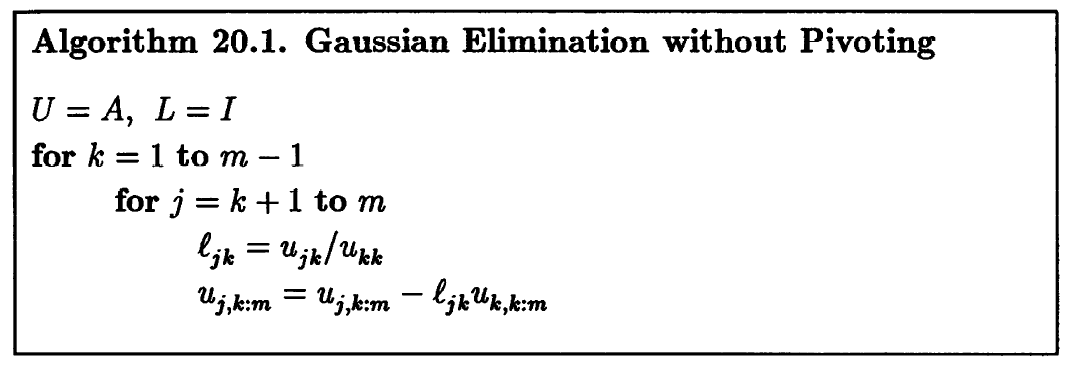
\includegraphics[width = 0.7\textwidth]{figs/TB97_Guass_wo_piv}
    \end{figure}
    \item Apply this loop at the matrix $A$ and obtain the $L$ and $U$ matrices.
\end{enumerate}

\subsection{}
Use the LU factorization to solve the linear system $Ax=b$ with
  $b=[1, 0, 0]^\top$ using one forward and one backward substitution.
  
\subsection{}\label{sec:1c}
Use the LU factorization to compute the determinant of
  $A$. Recall that for two matrices of appropriate sizes,
  $\det(AB)=\det(A)\det(B)$.
  

\newpage
\section{Block matrices and MATLAB matrix operations}
\subsection{}
Let's practice creating matrices in the computer:
\begin{enumerate}
    \item Create a matrix of all ones in your favorite coding language.
    \item Create a matrix where its entries are independent standard Gaussian random variables (i.e.: with density $\mcal{N}(0,1)$). 
\end{enumerate}

\subsection{}
Now let's operate on these matrices:
\begin{enumerate}
    \item Sum two matrices.
    \item Multiply a matrix with an appropriately sized vector.
    \item Multiply two matrices (Try some non-square matrices).
\end{enumerate}

\subsection{}
Suppose we split up a matrix of size $\mathbb{R}^{(m+n)\times(m+n)}$ into blocks:
\begin{align*}
    A = \left[\begin{array}{c|c} A_{11} & A_{12} \\\hline A_{21} & A_{22} \end{array}\right]
\end{align*}
where $A_{11}\in\mathbb{R}^{n\times n}$, $A_{22}\in\mathbb{R}^{m\times m}$, $A_{12}\in\mathbb{R}^{n\times m}$, and $A_{21}\in\mathbb{R}^{m\times n}$. 

We have the block matrix multiplication formula:
\begin{align*}
    AB = \left[
\begin{array}{c|c} A_{11} & A_{12} \\\hline A_{21} & A_{22} \end{array} \right]\cdot
\left[
\begin{array}{c|c} B_{11} & B_{12} \\\hline B_{21} & B_{22} \end{array} \right]
= 
\left[
\begin{array}{c|c} A_{11}B_{11}+A_{12}B_{21} & A_{11}B_{12}+A_{12}B_{22} \\\hline A_{21}B_{11}+A_{22}B_{21} & A_{21}B_{12}+A_{22}B_{22} \end{array} \right]
\end{align*}

You could try to prove this at home. In session we will verify this formula numerically by creating examples of $A$ and $B$.

\begin{enumerate}
    \item Make $A$ and $B$ to be Gaussian random matrices.
    \item How do you compare two matrices numerically?
\end{enumerate}

\subsection{}
(Challenge for you) Could you calculate the determinant of $A\in \mathbb{R}^{(m+n)\times(m+n)}$ by calculating the determinants of only $m$-by-$m$ and $n$-by-$n$ matrices? 

Hint: try Gaussian elimination on block matrices. Then follow the procedure in \ref{sec:1c}.


\newpage
\bibliographystyle{alpha}
\bibliography{citation}


\end{document}